\documentclass{beamer}
\colorlet{structure}{green!50!black}

\mode<article> % only for the article version
{
  \usepackage{fullpage}
  \usepackage{hyperref}
}
\mode<presentation>
{
	\setbeamertemplate{background canvas}[vertical shading][bottom=red!10,top=blue!10]
%	\useinnertheme[shadow=true]{rounded}
%	\useoutertheme{shadow}
%	\usecolortheme{whale}
	\setbeamerfont{block title}{size={}}
  \usefonttheme[onlysmall]{structurebold}
}

\setbeamersize{mini frame size=5cm}

\usepackage[english]{varioref}

\usetheme{Hannover}
\usecolortheme{dove}
%\setbeamercolor{math text}{fg=green!50!black}
%\setbeamercolor{normal text in math text}{parent=math text}

%\usepackage{pgf,pgfarrows,pgfnodes,pgfautomata,pgfheaps,pgfshade}
\usepackage{amsmath,amssymb}
%\usepackage[latin1]{inputenc}
\usepackage[utf8]{inputenc}
\usepackage{colortbl}
\usepackage[english,german,ngerman]{babel}
% Line spacing
\usepackage{setspace}
\usepackage{listings}
%\usepackage{lmodern}
%\usepackage[T1]{fontenc}
\usepackage{times}
\setbeamercovered{dynamic}

%
% The following defintions are peculiar to this particular
% presetation. They have nothing to do with the beamer class
%

\newcommand{\Lang}[1]{\operatorname{\text{\textsc{#1}}}}

\newcommand{\Class}[1]{\operatorname{\mathchoice
  {\text{\normalfont\small #1}}
  {\text{\normalfont\small #1}}
  {\text{\normalfont#1}}
  {\text{\normalfont#1}}}}

\newcommand{\DOF}{\Class{DOF}}
\newcommand{\NOF}{\Class{NOF}}
\newcommand{\DOFpoly}{\Class{DOF}_{\operatorname{poly}}}
\newcommand{\NOFpoly}{\Class{NOF}_{\operatorname{poly}}}

\newcommand{\Nat}{\mathbb{N}}
\newcommand{\Set}[1]{\{#1\}}

\newenvironment{ccodelisting}
{\begin{list}{}{\setlength{\leftmargin}{1em}}\item\scriptsize\bfseries}
{\end{list}}


%
% The following info should normally be given in you main file:
%
%\subject{cryptographic primitives}
%\lstset{
%	language=ADA,
%        basicstyle=\ttfamily,
%        keywordstyle=\color{Red},
%        commentstyle=\color{Blue},
%        stringstyle=\color{Green},
%        showstringspaces=false,
%        emph={bool,int,unsigned,char,true,false,void}, %emphstyle=\color{CornflowerBlue},
%        emph={[2]IFF\_TUN}, emphstyle={[2]\color{red}}
%}

\author{S\"oren Heisrath \and Daniel Otte}
\title{AnonAccess}
\institute{\includegraphics[scale=0.25]{laborlogo.png}}
\date[21. Dezember 2007]{21.12.2007}

\begin{document}

%-------------------------------------------------------------------------------

\frame{\titlepage}

\section<presentation>*{}

\begin{frame}
  \frametitle{}
  \tableofcontents[part=1,pausesection,hideallsubsections]
\end{frame}

%\AtBeginSubsection[]
%\AtBeginSection[]
%{
%  \begin{frame}<beamer>
%    \frametitle{"Ubersicht}
%    \tableofcontents[currentsection]
%    %\tableofcontents[current,currentsubsection]
%  \end{frame}
%}

\part<presentation>{Intro}
\section{Anforderungen \& Beispiele}
\begin{frame}
\frametitle{Anforderungen}
	\begin{itemize}
		\item<2-> Wartbarkeit
		\item<3-> Kryptografische Sicherheit
		\item<4-> Physikalische Sicherheit
		\item<5-> Kleines \& Energieeffizientes System
		\item<6-> Anonymit"at
	\end{itemize}
\end{frame}
\begin{frame}
\frametitle{Wartbarkeit}
	\begin{itemize}
		\item<2-> Hinzuf"ugen von Nutzern
		\item<3-> L"oschen von Nutzern
		\item<4-> Privilegien verwalten
	\end{itemize}
\end{frame}
\begin{frame}
\frametitle{Kryptografische Sicherheit}
	\begin{itemize}
		\item<2-> Sicherung des Kanals
		\item<3-> Sichere Speicherung der Datenbank
		\item<4-> Kryptografisch sicherer Zufallsgenerator
	\end{itemize}
\end{frame}

\begin{frame}
\frametitle{Physikalische Sicherheit}
	\begin{itemize}
		\item<2-> Sicherung gegen "offnen des Geh"auses
		\item<3-> Sichere L"oschung der Daten
	\end{itemize}
\end{frame}

\begin{frame}
\frametitle{Hardwareanforderungen}
	\begin{itemize}
		\item<2-> Microcontroller Plattform
		\item<3-> USV Sicherung f"ur mehrere Tage
	\end{itemize}
\end{frame}

\section{Aufbau}
\begin{frame}
	\frametitle{Grundaufbau}
	\begin{center}
		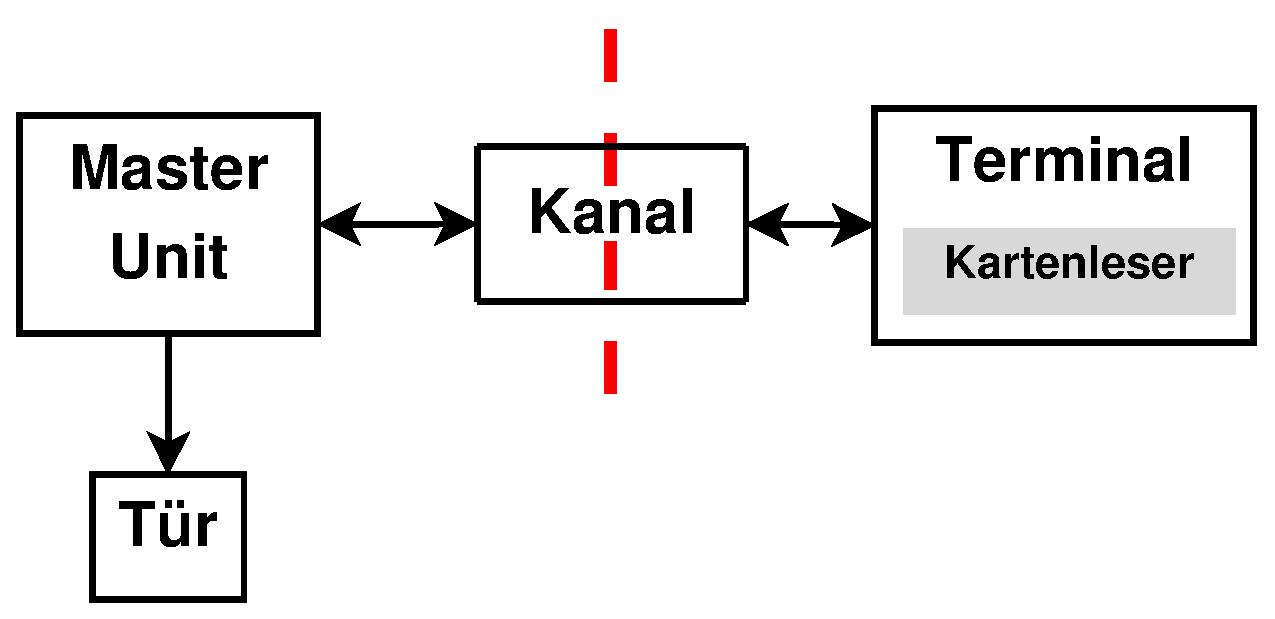
\includegraphics[width=210px]{grundaufbau}
	\end{center}
\end{frame}

\begin{frame}
	\frametitle{Master Unit}
	\begin{itemize}
		\item<2-> Speicherung der Datenbank
		\item<3-> Authentifizierung der Nutzer
		\item<4-> L"oschung der Schl"ussel \& Datenbank bei physikalischen Angriffen
		\item<5-> USV
	\end{itemize}
\end{frame}

\begin{frame}
	\frametitle{Panel}
	\begin{itemize}
		\item<2-> Weitergabe der Kartendaten
		\item<3-> Ein- und Ausgabe \small{(Master Unit <-> Mensch)}
		\item<4-> L"oschung des Schl"ussels bei physikalischen Angriffen
	\end{itemize}
\end{frame}

\begin{frame}
	\frametitle{Kanal}
	Galvanische Trennung zwischen Master Unit und Panel
\end{frame}

\section{Begriffe}
\begin{frame}
	\frametitle{Token}
	\vspace{1cm}
	Einmal verwendbarer Datensatz zur Authentifikation
\end{frame}


%
% TODO: add lots of photos ;-)
%

\section{Implementation}

\begin{frame}
	\frametitle{Zus"atzliche Hardwareanforderungen}
	\begin{itemize}
		\item<2-> Microcontroller Plattform
		\item<3-> USV Sicherung f"ur mehrere Tage
		\item<4-> Physikalische Sicherung gegen das Auslesen der Datenbank
	\end{itemize}
\end{frame}

%
%
%   .....
%

% TODO
%
% >> hardware sektion vervollstaendigen
%

\section{Komponenten}
\begin{frame}
	\frametitle{Hardware}
	\textbf{Microcontroller:}
	\begin{itemize}
		\item Atmel Atmega 32
		\item Atmel Atmega 644
	\end{itemize}
	\par
	\textbf{i^2c Speicher-Chipkarten} mit 256 Byte Speicherkapazit"at
	\par
	\textbf{Optokoppler} (Laserdioden \& Fototransistoren aus altem Switch)
	\par
	\textbf{i^2c EEPROM} (insert vendor \& name here.)
	\par
	\textbf{Kartenleser} (Ausgeschlachtet aus ??)
\end{frame}

\begin{frame}
	\frametitle{Software}
	\begin{itemize}
		\item AVR-GCC
		\item Crypto AVR Lib (Daniel Otte)
		\item Programmiert in C
	\end{itemize}
\end{frame}

\section{Varianten zur Verwaltung}

\begin{frame}
	\frametitle{Identifizierung durch Nicknames}
	\begin{itemize}
		\item Wartbare M"oglichkeit
		\item Nicht ganz so anonym
	\end{itemize}
\end{frame}

\begin{frame}
	\frametitle{Anonymer Zugang}
	\begin{itemize}
		\item Nur durch Timeouts wartbar
		\item Anonym
	\end{itemize}
\end{frame}

% ----

\end{document}

